% Delhi PM2.5: progress presentation, MATH F428.
% Build: python make_figures.py && tectonic main.tex   (numbers in the slides come from tables/numbers.tex)
\documentclass[aspectratio=169,11pt]{beamer}
\usepackage{graphicx}
\usepackage{tikz}
\usetikzlibrary{positioning,arrows.meta,shapes.misc,calc}
\usepackage{booktabs}
\usepackage[most]{tcolorbox}
\usepackage{hyperref}
\hypersetup{colorlinks=true,urlcolor=blue!70!black,linkcolor=blue!70!black}

% ── palette (same blue / orange / aqua as the figures) ─────────────────────────────────────────────────
\definecolor{navy}{HTML}{12284C}
\definecolor{pblue}{HTML}{2A78D6}
\definecolor{porange}{HTML}{EB6834}
\definecolor{paqua}{HTML}{1BAF7A}
\definecolor{pgreen}{HTML}{2E8B57}
\definecolor{lightbg}{HTML}{EEF3FA}
\definecolor{graytxt}{HTML}{5B6573}

\usetheme{default}
\usefonttheme{professionalfonts}
\setbeamertemplate{navigation symbols}{}
\setbeamercolor{normal text}{fg=black}
\setbeamercolor{structure}{fg=pblue}
\setbeamercolor{frametitle}{bg=navy,fg=white}
\setbeamerfont{frametitle}{size=\large,series=\bfseries}
\setbeamersize{text margin left=0.7cm,text margin right=0.7cm}
\setbeamertemplate{itemize item}{\color{pblue}$\blacktriangleright$}
\setbeamertemplate{itemize subitem}{\color{pblue}$\bullet$}
\setlength{\leftmargini}{1.1em}

% slim navy title bar
\setbeamertemplate{frametitle}{%
  \nointerlineskip
  \begin{beamercolorbox}[wd=\paperwidth,ht=0.85cm,dp=0.25cm,leftskip=0.7cm]{frametitle}
    \usebeamerfont{frametitle}\insertframetitle
  \end{beamercolorbox}\vspace{0.05cm}}

% footer: course | topic, small logo, page number
\setbeamertemplate{footline}{%
  \leavevmode\hbox to\paperwidth{%
    \hspace*{0.7cm}\raisebox{0.12cm}{\color{graytxt}\tiny MATH F428 $\cdot$ Delhi PM$_{2.5}$ forecasting $\cdot$ K.\ Singh, Y.\ JM, A.\ Choudhary (BITS Goa)}\hfill
    \raisebox{0.03cm}{
\includegraphics[height=0.36cm]{logo.png}}\hspace*{0.25cm}%
    \raisebox{0.12cm}{\color{graytxt}\tiny\insertframenumber\,/\,\inserttotalframenumber}\hspace*{0.7cm}}%
  \vskip0.04cm}

% boxes: definition (light), takeaway (navy)
\newtcolorbox{defbox}[1]{enhanced,colback=lightbg,colframe=pblue,boxrule=0pt,leftrule=2.5pt,arc=1pt,
  left=5pt,right=5pt,top=2pt,bottom=2pt,before skip=3pt,after skip=3pt,fontupper=\footnotesize,
  before upper={\textbf{\textcolor{pblue}{#1}}\;}}
\newtcolorbox{takeaway}{enhanced,colback=navy,colupper=white,boxrule=0pt,arc=2pt,
  left=6pt,right=6pt,top=3pt,bottom=3pt,before skip=3pt,after skip=0pt,fontupper=\small}
\newtcolorbox{card}[2][]{enhanced,colback=white,colframe=#2,coltitle=white,colbacktitle=#2,boxrule=0.6pt,
  arc=2pt,fonttitle=\bfseries\small,fontupper=\small,left=5pt,right=5pt,top=3pt,bottom=3pt,#1}

\tikzset{
  sbox/.style={draw=#1,rounded corners=2pt,line width=0.9pt,fill=white,align=left,inner sep=4pt,text width=5.1cm,minimum height=1.25cm},
  sres/.style={draw=#1,rounded corners=2pt,line width=0.9pt,fill=#1!8,align=left,inner sep=4pt,text width=4.0cm,minimum height=1.25cm},
  gbox/.style={draw=#1,rounded corners=2pt,fill=#1!8,line width=0.8pt,align=center,inner sep=3pt,text width=3.9cm},
  sarr/.style={-{Stealth[length=2.2mm]},line width=0.9pt,color=graytxt}}
\newcommand{\pmtwo}{PM$_{2.5}$}
\newcommand{\ugm}{$\mu$g/m$^3$}
\renewcommand{\arraystretch}{1.1}
\setlength{\parskip}{0pt}\setlength{\parindent}{0pt}
\newcommand{\nDays}{2{,}009}
\newcommand{\nWeeks}{287}
\newcommand{\nWeeksModel}{261}
\newcommand{\nTrain}{209}
\newcommand{\pctPoor}{54}
\newcommand{\pmMean}{121}
\newcommand{\winterMean}{217}
\newcommand{\monsoonMean}{48}
\newcommand{\ratioWM}{4.5}
\newcommand{\skewRaw}{1.66}
\newcommand{\skewLog}{\ensuremath{-}0.14}
\newcommand{\corrRaw}{0.94}
\newcommand{\corrLog}{\ensuremath{-}0.09}
\newcommand{\sdRatioRaw}{7.9}
\newcommand{\sdRatioLog}{1.5}
\newcommand{\Fs}{0.90}
\newcommand{\Ft}{0.18}
\newcommand{\seasRatio}{17}
\newcommand{\declAll}{22}
\newcommand{\acfOne}{0.87}
\newcommand{\acfHalf}{\ensuremath{-}0.43}
\newcommand{\acfYear}{0.68}
\newcommand{\acfDOne}{0.29}
\newcommand{\adfPLog}{\ensuremath{4.8\times10^{-4}}}
\newcommand{\kpssLog}{0.058}
\newcommand{\adfPDiff}{\ensuremath{1.7\times10^{-4}}}
\newcommand{\kpssDiff}{0.341}
\newcommand{\stnFirst}{10}
\newcommand{\stnSecond}{8}
\newcommand{\stnLast}{37}
\newcommand{\varLagAic}{4}
\newcommand{\varLagBic}{2}
\newcommand{\portP}{0.17}
\newcommand{\spearWind}{\ensuremath{-}0.22}
\newcommand{\spearRh}{\ensuremath{-}0.26}
\newcommand{\gWindP}{\ensuremath{<10^{-12}}}
\newcommand{\gRhP}{\ensuremath{1.2\times10^{-11}}}
\newcommand{\gBothP}{\ensuremath{<10^{-12}}}
\newcommand{\gRevWindP}{0.12}
\newcommand{\gRevRhP}{0.62}
\newcommand{\gWindPc}{\ensuremath{<10^{-12}}}
\newcommand{\gRhPc}{\ensuremath{9.7\times10^{-9}}}
\newcommand{\nestRone}{0.123}
\newcommand{\nestRtwo}{0.128}
\newcommand{\nestDR}{0.005}
\newcommand{\nestP}{0.47}
\newcommand{\nestRsame}{0.17}
\newcommand{\sarMA}{\ensuremath{-}0.99}
\newcommand{\sarMASE}{8}
\newcommand{\lbAll}{\ensuremath{<10^{-12}}}
\newcommand{\lbTen}{0.49}
\newcommand{\lbTwentySix}{0.10}
\newcommand{\lbFiftyTwo}{0.016}
\newcommand{\maeNaiveSeventeen}{38.4}
\newcommand{\maeNaiveEighteen}{29.0}
\newcommand{\maeNaiveNineteen}{30.3}
\newcommand{\maeNaiveAvg}{29.6}
\newcommand{\rmseNaiveAvg}{43.1}
\newcommand{\mapeNaiveAvg}{30}
\newcommand{\meNaiveAvg}{\ensuremath{-}8.1}
\newcommand{\covNaiveSeventeen}{88}
\newcommand{\covNaiveEighteen}{94}
\newcommand{\covNaiveNineteen}{92}
\newcommand{\maeMeanSeventeen}{31.0}
\newcommand{\maeMeanEighteen}{21.8}
\newcommand{\maeMeanNineteen}{27.8}
\newcommand{\maeMeanAvg}{24.8}
\newcommand{\rmseMeanAvg}{34.7}
\newcommand{\mapeMeanAvg}{27}
\newcommand{\meMeanAvg}{\ensuremath{-}10.8}
\newcommand{\covMeanSeventeen}{62}
\newcommand{\covMeanEighteen}{92}
\newcommand{\covMeanNineteen}{81}
\newcommand{\maeHWSeventeen}{44.7}
\newcommand{\maeHWEighteen}{19.2}
\newcommand{\maeHWNineteen}{32.2}
\newcommand{\maeHWAvg}{25.7}
\newcommand{\rmseHWAvg}{36.1}
\newcommand{\mapeHWAvg}{30}
\newcommand{\meHWAvg}{\ensuremath{-}14.7}
\newcommand{\covHWSeventeen}{64}
\newcommand{\covHWEighteen}{94}
\newcommand{\covHWNineteen}{86}
\newcommand{\maeSarimaSeventeen}{72.3}
\newcommand{\maeSarimaEighteen}{21.1}
\newcommand{\maeSarimaNineteen}{27.5}
\newcommand{\maeSarimaAvg}{24.3}
\newcommand{\rmseSarimaAvg}{34.5}
\newcommand{\mapeSarimaAvg}{27}
\newcommand{\meSarimaAvg}{\ensuremath{-}11.7}
\newcommand{\covSarimaSeventeen}{23}
\newcommand{\covSarimaEighteen}{94}
\newcommand{\covSarimaNineteen}{85}
\newcommand{\maeHarmSeventeen}{29.4}
\newcommand{\maeHarmEighteen}{22.5}
\newcommand{\maeHarmNineteen}{26.4}
\newcommand{\maeHarmAvg}{24.5}
\newcommand{\rmseHarmAvg}{34.0}
\newcommand{\mapeHarmAvg}{26}
\newcommand{\meHarmAvg}{\ensuremath{-}10.7}
\newcommand{\covHarmSeventeen}{65}
\newcommand{\covHarmEighteen}{92}
\newcommand{\covHarmNineteen}{86}
\newcommand{\maeCombSeventeen}{38.2}
\newcommand{\maeCombEighteen}{20.1}
\newcommand{\maeCombNineteen}{27.6}
\newcommand{\maeCombAvg}{23.8}
\newcommand{\rmseCombAvg}{33.7}
\newcommand{\mapeCombAvg}{27}
\newcommand{\meCombAvg}{\ensuremath{-}11.8}
\newcommand{\dmPNaive}{0.03}
\newcommand{\dmDNaive}{4.8}
\newcommand{\dmPHW}{0.57}
\newcommand{\dmDHW}{0.9}
\newcommand{\dmPSarima}{0.49}
\newcommand{\dmDSarima}{\ensuremath{-}0.5}
\newcommand{\dmPHarm}{0.74}
\newcommand{\dmDHarm}{\ensuremath{-}0.3}
\newcommand{\dmPComb}{0.08}
\newcommand{\dmDComb}{\ensuremath{-}0.9}
\newcommand{\covMinSeventeen}{23}
\newcommand{\covMaxSeventeen}{88}
\newcommand{\covMinEighteen}{92}
\newcommand{\covMaxEighteen}{94}
\newcommand{\covMinNineteen}{81}
\newcommand{\covMaxNineteen}{92}
\newcommand{\bestAvgModel}{Combination}
\newcommand{\widthNaiveNineteen}{160}
\newcommand{\widthNaiveSeventeen}{167}
\newcommand{\widthMeanNineteen}{103}
\newcommand{\widthMeanSeventeen}{77}
\newcommand{\widthHWNineteen}{173}
\newcommand{\widthHWSeventeen}{131}
\newcommand{\widthSarimaNineteen}{133}
\newcommand{\widthSarimaSeventeen}{36}
\newcommand{\widthHarmNineteen}{112}
\newcommand{\widthHarmSeventeen}{90}
\newcommand{\hwGamma}{\ensuremath{7.3\times10^{-5}}}
\newcommand{\hwAlpha}{0.27}
\newcommand{\onePers}{30.7}
\newcommand{\oneMean}{24.8}
\newcommand{\oneNo}{21.5}
\newcommand{\oneLag}{22.1}
\newcommand{\oneOracle}{20.0}
\newcommand{\oneLagPct}{2.6}
\newcommand{\oneOraclePct}{\ensuremath{-}7.2}
\newcommand{\oneLagP}{0.04}
\newcommand{\oneOracleP}{0.08}
\newcommand{\lockActual}{49}
\newcommand{\lockFcHarm}{95}
\newcommand{\lockFcMean}{97}
\newcommand{\lockGapHarm}{\ensuremath{-}49}
\newcommand{\lockGapMean}{\ensuremath{-}50}
\newcommand{\lockGapMin}{\ensuremath{-}44}
\newcommand{\lockGapMax}{\ensuremath{-}50}
\newcommand{\lockPreHarm}{\ensuremath{-}16}
\newcommand{\lockAdjMin}{\ensuremath{-}34}
\newcommand{\lockAdjMax}{\ensuremath{-}41}
\newcommand{\lockAdjHarm}{\ensuremath{-}39}
\newcommand{\lockPlaceboHarm}{\ensuremath{-}14}
\newcommand{\janMaeMin}{28}
\newcommand{\janMaeMax}{42}
\newcommand{\preBiasLo}{7}
\newcommand{\preBiasHi}{17}
\newcommand{\preBiasMin}{\ensuremath{-}7}
\newcommand{\preBiasMax}{\ensuremath{-}17}
\newcommand{\janMaeHarm}{35.7}
\newcommand{\janMaeMean}{36.4}
\newcommand{\lockUsualLo}{\ensuremath{-}31}
\newcommand{\lockUsualHi}{23}
\newcommand{\lockWinMinHarm}{\ensuremath{-}36}
\newcommand{\lockWinMin}{\ensuremath{-}52}
\newcommand{\lockWinMax}{42}
\newcommand{\exWeek}{3}
\newcommand{\exYa}{188}
\newcommand{\exYb}{272}
\newcommand{\exYc}{238}
\newcommand{\exYd}{197}
\newcommand{\exMean}{221}
\newcommand{\exNaive}{197}
\newcommand{\declWeeks}{26}
\newcommand{\aicA}{73.2}
\newcommand{\aicB}{53.9}
\newcommand{\aicC}{39.4}
\newcommand{\aicD}{45.2}
\newcommand{\aicE}{57.5}
\newcommand{\aicBest}{39.4}
\newcommand{\aicGap}{5.8}
\newcommand{\kHarmLo}{6}
\newcommand{\kHarmHi}{7}
\newcommand{\lockShareHW}{3}
\newcommand{\lockShareAdjHW}{8}
\newcommand{\lockMinHW}{\ensuremath{-}46}
\newcommand{\lockShareSarima}{1}
\newcommand{\lockShareAdjSarima}{5}
\newcommand{\lockMinSarima}{\ensuremath{-}52}
\newcommand{\lockShareHarm}{0}
\newcommand{\lockShareAdjHarm}{0}
\newcommand{\lockMinHarm}{\ensuremath{-}36}
\newcommand{\lockShareMean}{0}
\newcommand{\lockShareAdjMean}{0}
\newcommand{\lockMinMean}{\ensuremath{-}36}


\title{Forecasting Delhi's PM$_{2.5}$ Air Pollution}
\author{Kushagra Singh \and Yatin JM \and Aryan Choudhary}
\date{October 2026}

\begin{document}

% ───────────────────────── 1. Title ─────────────────────────
\begin{frame}[plain]
  \begin{tikzpicture}[remember picture,overlay]
    \fill[navy] (current page.south west) rectangle (current page.north east);
    \fill[porange] ([xshift=0.9cm,yshift=-2.15cm]current page.north west) rectangle +(1.4cm,0.09cm);
    \node[anchor=north west,text=white,text width=12cm,inner sep=0] at ([xshift=0.9cm,yshift=-2.4cm]current page.north west)
      {{\fontsize{24}{28}\selectfont\bfseries Forecasting Delhi's PM$_{2.5}$\\[2pt] Air Pollution}\\[8pt]
       {\large Time-series analysis with VAR, Granger causality and SARIMA}\\[14pt]
       {\normalsize Kushagra Singh \;$\cdot$\; Yatin JM \;$\cdot$\; Aryan Choudhary}\\[3pt]
       {\small BITS Pilani, Goa \;$\cdot$\; MATH F428 Project Presentation \;$\cdot$\; October 2026}};
    \node[anchor=south west,text=white!85!navy,text width=10cm,inner sep=0] at ([xshift=0.9cm,yshift=0.8cm]current page.south west)
      {\small Can weather explain Delhi's smog, and can we forecast it a year ahead?};
    \node[anchor=north east,fill=white,circle,inner sep=2pt] at ([xshift=-0.8cm,yshift=-0.8cm]current page.north east)
      {
\includegraphics[height=1.5cm]{logo.png}};
  \end{tikzpicture}
\end{frame}

% ───────────────────────── 2. The problem ─────────────────────────
\begin{frame}{The Problem: Delhi's Air Is Unhealthy Most of the Year}
  \centering
  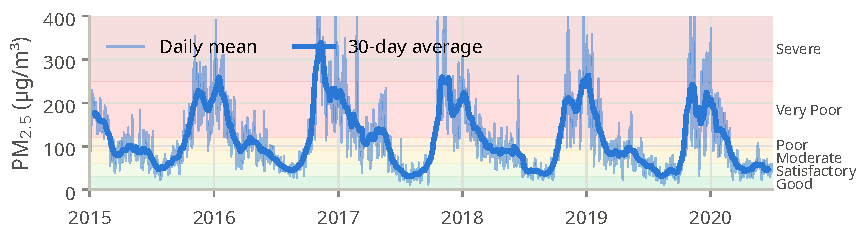
\includegraphics[width=\linewidth]{fig/problem_aqi.pdf}\\[3pt]
  \begin{defbox}{PM$_{2.5}$ and AQI:}
    particles under 2.5 $\mu$m that reach the lungs and blood, in \ugm{} (micrograms per m$^3$). \textbf{AQI} = India's colour-coded Air Quality Index; the bands show its PM$_{2.5}$ categories (Poor starts above 90 \ugm{}).
  \end{defbox}
  \begin{takeaway}
    \textbf{\pctPoor\%} of days (2015--2020) were Poor or worse, and the pattern repeats yearly: winter averages \textbf{\winterMean} \ugm{}, the monsoon \textbf{\monsoonMean}: winter is \textbf{\ratioWM$\times$} higher.
  \end{takeaway}
\end{frame}

% ───────────────────────── 3. What we are building ─────────────────────────
\begin{frame}{What We Are Building: Two Questions, Two Time Horizons}
  \centering
  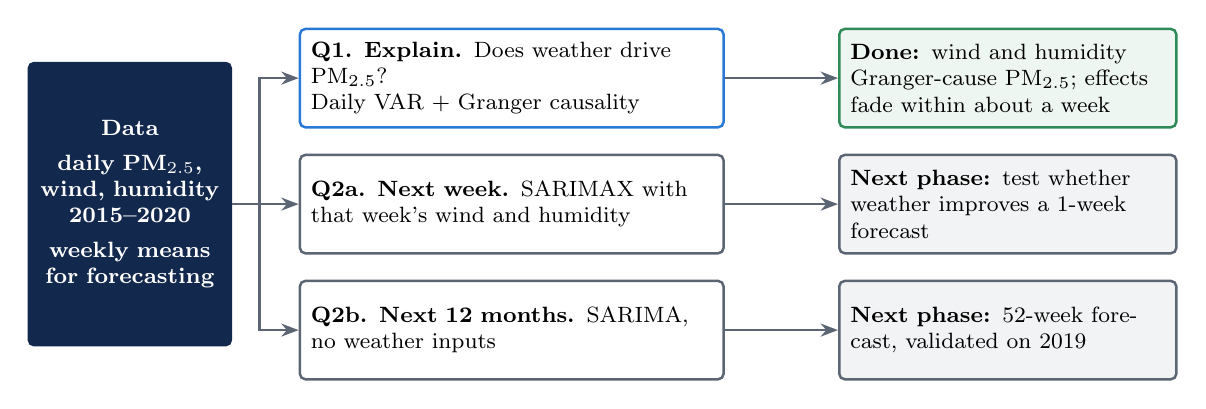
\begin{tikzpicture}[x=1cm,y=1cm,font=\footnotesize]
    \node[draw=navy,fill=navy,text=white,rounded corners=2pt,align=center,text width=2.3cm,minimum height=3.6cm,inner sep=4pt] (data)
      at (1.15,2.0) {\bfseries Data\\[3pt]\footnotesize daily \pmtwo{}, wind, humidity\\ 2015--2020\\[3pt] weekly means for forecasting};
    \node[sbox=pblue] (q1) at (6.0,3.6) {\textbf{Q1. Explain.} Does weather drive \pmtwo{}?\\ Daily VAR + Granger causality};
    \node[sbox=graytxt] (q2a) at (6.0,2.0) {\textbf{Q2a. Next week.} SARIMAX with that week's wind and humidity};
    \node[sbox=graytxt] (q2b) at (6.0,0.4) {\textbf{Q2b. Next 12 months.} SARIMA, no weather inputs};
    \node[sres=pgreen] (r1) at (12.3,3.6) {\textbf{Done:} wind and humidity Granger-cause \pmtwo{}; effects fade within about a week};
    \node[sres=graytxt] (r2) at (12.3,2.0) {\textbf{Next phase:} test whether weather improves a 1-week forecast};
    \node[sres=graytxt] (r3) at (12.3,0.4) {\textbf{Next phase:} 52-week forecast, validated on 2019};
    \draw[sarr] (data.east) -- ++(0.35,0) |- (q1.west);
    \draw[sarr] (data.east) -- (q2a.west);
    \draw[sarr] (data.east) -- ++(0.35,0) |- (q2b.west);
    \draw[sarr] (q1) -- (r1); \draw[sarr] (q2a) -- (r2); \draw[sarr] (q2b) -- (r3);
  \end{tikzpicture}\\[4pt]
  \begin{takeaway}
    \textbf{Why two horizons?} Q1 shows a weather shock moves \pmtwo{} for only about a week: weather may help a short-term forecast, but it is unknown a year ahead, so the 12-month model will use no weather inputs.
    The final output is a month-by-month AQI outlook for health advisories.
  \end{takeaway}
\end{frame}

% ───────────────────────── 4. Data ─────────────────────────
\begin{frame}{Data: CPCB Air Quality and ERA5 Weather}
  \footnotesize
  \begin{tabular}{@{}p{3.7cm}p{1.8cm}p{1.1cm}p{6.6cm}@{}}
    \toprule
    \textbf{Variable} & \textbf{Source} & \textbf{Unit} & \textbf{Role in the project} \\
    \midrule
    \pmtwo{} & CPCB & \ugm{} & What we explain and forecast \\
    Wind speed & ERA5 & km/h & Disperses pollution: candidate driver \\
    Relative humidity & ERA5 & \% & Moisture, fog, rain: candidate driver \\
    Other (NO$_2$, SO$_2$, temp., rain) & CPCB, ERA5 & various & Context; rain used as a control \\
    \bottomrule
  \end{tabular}\\[5pt]
  \footnotesize
  \begin{itemize}\setlength\itemsep{2pt}
    \item \textbf{CPCB} (India's pollution board): \href{https://www.kaggle.com/datasets/rohanrao/air-quality-data-in-india}{\textbf{Kaggle: Air Quality Data in India}}, Delhi rows.
    \item \textbf{ERA5} = a \emph{reanalysis} (observations blended into a weather model, gap-free): \href{https://open-meteo.com/en/docs/historical-weather-api}{\textbf{Open-Meteo Historical API}}, central Delhi.
    \item \textbf{2{,}009 days}, 1 Jan 2015 -- 1 Jul 2020; 2 \pmtwo{} values interpolated. \textbf{Daily} data for causality, \textbf{weekly means} (287 weeks) for forecasting.
  \end{itemize}
  \vspace{1pt}
  \centering
  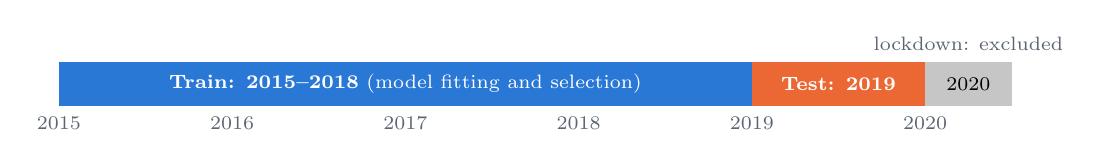
\begin{tikzpicture}[x=2.2cm,font=\scriptsize]
    \fill[pblue] (0,0) rectangle (4,0.55);        \node[text=white] at (2,0.275) {\textbf{Train: 2015--2018} (model fitting and selection)};
    \fill[porange] (4,0) rectangle (5,0.55);      \node[text=white] at (4.5,0.275) {\textbf{Test: 2019}};
    \fill[gray!45] (5,0) rectangle (5.5,0.55);    \node at (5.25,0.275) {2020};
    \foreach \y/\l in {0/2015,1/2016,2/2017,3/2018,4/2019,5/2020} \node[text=graytxt,anchor=north] at (\y,-0.02) {\l};
    \node[text=graytxt,anchor=south,align=center] at (5.25,0.58) {lockdown: excluded};
  \end{tikzpicture}
\end{frame}

% ───────────────────────── 5. Seasonality / STL ─────────────────────────
\begin{frame}{Seasonality: STL Decomposition of Weekly log PM$_{2.5}$}
  \centering
  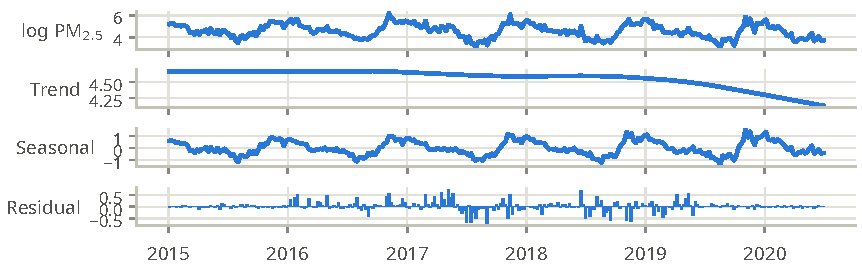
\includegraphics[width=\linewidth]{fig/stl.pdf}\\[3pt]
  \begin{defbox}{STL.}
    Splits a series into \emph{trend} + \emph{seasonal} (repeats every year) + \emph{residual} (what is left).
    Seasonal strength $F_S=1-\mathrm{Var}(\text{residual})/\mathrm{Var}(\text{seasonal}+\text{residual})$: 0 = no seasonality, 1 = purely seasonal.
  \end{defbox}
  \begin{takeaway}
    $F_S=\mathbf{\Fs}$: the yearly cycle dominates, so the model must be \textbf{seasonal} (period $s=52$ weeks).
  \end{takeaway}
\end{frame}

% ───────────────────────── 6. Why log ─────────────────────────
\begin{frame}{Why Take Logs? Raw PM$_{2.5}$ Is Spiky and Skewed}
  \centering
  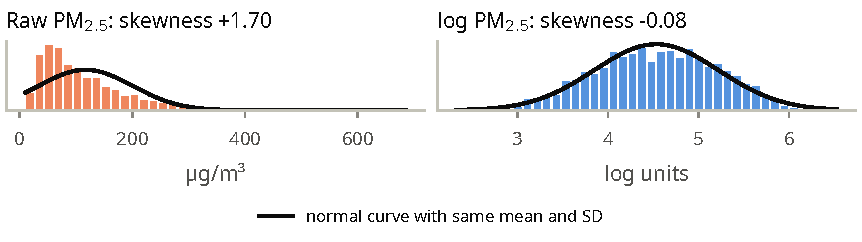
\includegraphics[width=\linewidth]{fig/why_log.pdf}\\[3pt]
  \begin{defbox}{Log transform.}
    PM$_{2.5}$ moves by \emph{percentages}: the spread of daily values (SD) is about \sdNov\ \ugm{} in November but only \sdAug\ in August. On a log scale equal percentage changes are equal distances, so the spread stops depending on the level.
  \end{defbox}
  \begin{takeaway}
    Raw PM$_{2.5}$ has a heavy right tail (skewness \skewRaw); the log is close to a bell curve (skewness \skewLog). The Box-Cox estimate $\lambda\approx\boxcox$ ($\lambda=0$ is the log) agrees.
  \end{takeaway}
\end{frame}

% ───────────────────────── 7. Volatility ─────────────────────────
\begin{frame}{Volatility Tests: Does the Spread Depend on the Level?}
  \centering
  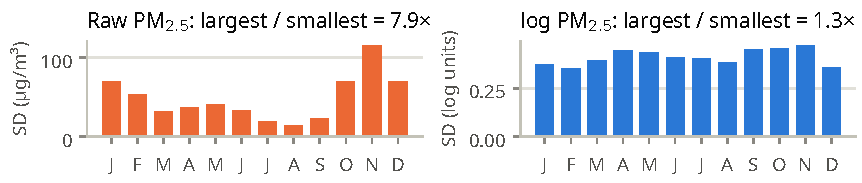
\includegraphics[width=\linewidth]{fig/volatility_sd.pdf}\\[2pt]
  {\scriptsize\begin{tabular}{lrr}
\toprule
\textbf{Question the test asks} & \textbf{Raw} & \textbf{Log} \\
\midrule
Does spread grow with level? (corr.\ of monthly mean and SD) & 0.95 & -0.07 \\
Is the spread equal in all 12 months? (Levene $F$) & 49.63 & 2.40 \\
Do big changes cluster in time? (ARCH-LM) & 235.18 & 36.43 \\
\bottomrule
\end{tabular}
}\\[3pt]
  \begin{takeaway}
    \textbf{Volatility} = how much values swing. In raw units the spread differs \sdRatioRaw$\times$ between months and tracks the level (corr.\ 0.95); after the log it differs only \sdRatioLog$\times$.
    Small differences remain (equal-spread test $p=\levPlog$; ARCH \archRaw\,$\to$\,\archLog, still significant), so we re-check the model residuals.
  \end{takeaway}
\end{frame}

% ───────────────────────── 8. Stationarity (idea) ─────────────────────────
\begin{frame}{Stationarity: Can the Past Predict the Future?}
  \centering
  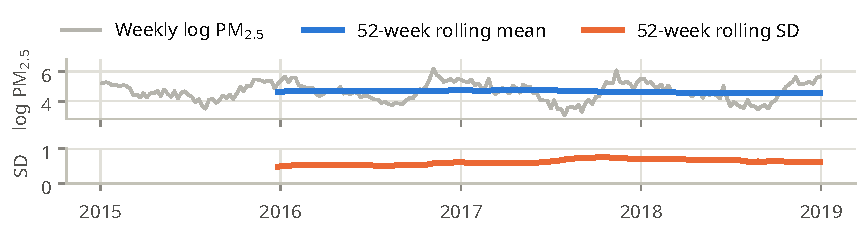
\includegraphics[width=\linewidth]{fig/stationarity.pdf}\\[3pt]
  \begin{defbox}{Stationary}
    = the mean, spread and autocorrelation do not drift over time, so patterns learned from the past still apply. ARIMA-type models need it; if a series drifts, we \emph{difference} it ($d$ = ordinary difference, $D$ = difference at the seasonal lag).
  \end{defbox}
  \begin{takeaway}
    Weekly log \pmtwo{} (2015--18): the rolling mean is flat and the rolling spread varies only modestly, so the yearly cycle is a repeating pattern, not a drifting trend. (Raw daily \pmtwo{} also passes ADF and KPSS in our checks: the log is for variance, not for stationarity.)
  \end{takeaway}
\end{frame}

% ───────────────────────── 8b. ADF / KPSS ─────────────────────────
\begin{frame}{Testing Stationarity with ADF and KPSS, and Choosing $d$ and $D$}
  \centering
  {\footnotesize\begin{tabular}{|l|r|r|r|r|r|}
\hline
\textbf{Weekly series, 2015--18} & \textbf{ADF stat} & \textbf{5\% crit.} & \textbf{ADF $p$} & \textbf{KPSS $p$} & \textbf{lag-1 ACF} \\\hline
log PM$_{2.5}$ (level) & -4.28 & -2.88 & $4.8\times10^{-4}$ & 0.10 & 0.87 \\\hline
seasonal difference $\Delta_{52}$ & -4.53 & -2.88 & $1.7\times10^{-4}$ & 0.10 & 0.29 \\\hline
$\Delta\Delta_{52}$ (over-differenced) & -7.30 & -2.88 & $1.4\times10^{-10}$ & 0.10 & -0.46 \\\hline
\end{tabular}
}\par\vspace{5pt}
  \begin{columns}[T,onlytextwidth]
    \column{0.485\linewidth}
    \begin{card}[title={ADF test (Augmented Dickey-Fuller)}]{pblue}\footnotesize
      H$_0$: \emph{unit root} (the series wanders, non-stationary).\\ $p<0.05$ rejects H$_0$, which supports stationarity.
    \end{card}
    \column{0.485\linewidth}
    \begin{card}[title={KPSS test}]{porange}\footnotesize
      H$_0$: the series \emph{is} stationary.\\ $p>0.05$ keeps H$_0$ (the printed 0.10 means ``$\ge0.10$'').
    \end{card}
  \end{columns}
  \vspace{4pt}
  \begin{takeaway}
    \textbf{Both tests pass} for log \pmtwo{} and for its seasonal difference $\Rightarrow$ $d=0$. A further difference over-differences (lag-1 autocorrelation $-0.46$, near the $-0.5$ warning level) and is dropped.
    \textbf{Seasonal difference $D$} (0 or 1) is chosen in the next phase, when we fit the seasonal models, using a validation year, not the test year.
  \end{takeaway}
\end{frame}

% ───────────────────────── 9. Granger ─────────────────────────
\begin{frame}{Does Weather Predict PM$_{2.5}$? Granger Causality in a VAR}
  \centering
  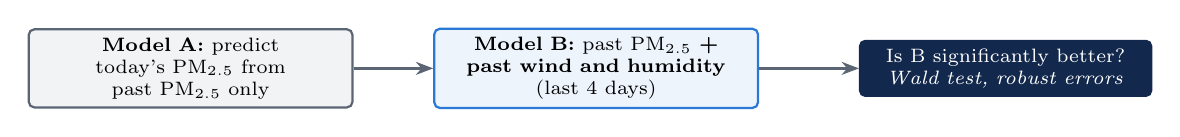
\begin{tikzpicture}[font=\scriptsize]
    \node[gbox=graytxt] (a) at (2.15,0) {\textbf{Model A:} predict today's \pmtwo{} from\\ past \pmtwo{} only};
    \node[gbox=pblue] (b) at (7.3,0) {\textbf{Model B:} past \pmtwo{} \textbf{+ past wind and humidity}\\(last 4 days)};
    \node[draw=navy,rounded corners=2pt,fill=navy,text=white,align=center,inner sep=3pt,text width=3.5cm] (c) at (12.5,0) {Is B significantly better?\\ \emph{Wald test, robust errors}};
    \draw[sarr] (a) -- (b); \draw[sarr] (b) -- (c);
  \end{tikzpicture}\\[3pt]
  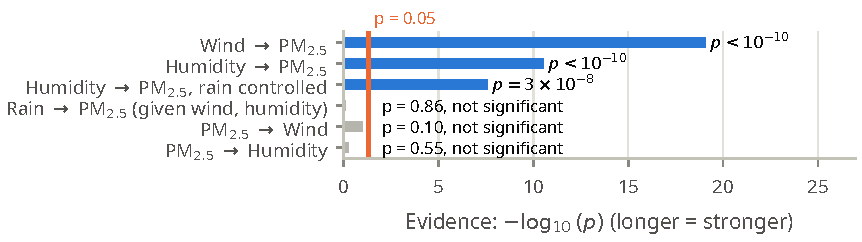
\includegraphics[width=\linewidth]{fig/granger_hac.pdf}\\[2pt]
  \begin{takeaway}
    \textbf{Mainly one way.} Wind and humidity help predict \pmtwo{} at every lag from 1 to 7 days ($p<10^{-9}$; bars: 4 lags), and humidity still matters given rain. The reverse is absent for humidity and weak for wind (lags 1--2 only, $p\approx0.02$--$0.04$). {\footnotesize Predictive, not proof of cause.}
  \end{takeaway}
\end{frame}

% ───────────────────────── 10. Shock ─────────────────────────
\begin{frame}{What Is a ``Shock''? An Unexpected Change in Weather}
  \centering
  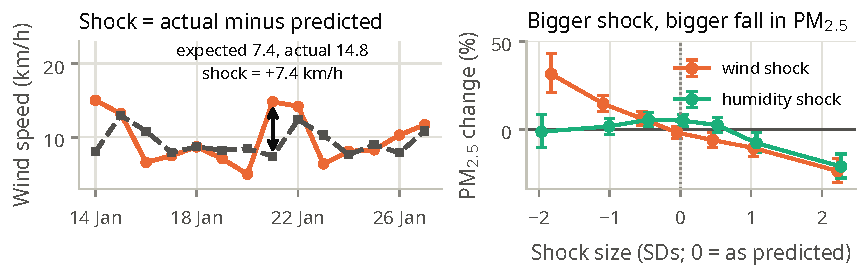
\includegraphics[width=\linewidth]{fig/shock_example.pdf}\\[3pt]
  \begin{defbox}{Shock.}
    the part of today's wind (or humidity) the model could \emph{not} predict from the previous 4 days (plus the seasonal level). \textbf{SD} = typical shock size: 1 SD $\approx$ 2.5 km/h (wind), 5.4\% (humidity).
  \end{defbox}
  \begin{takeaway}
    Grouping all days by shock size: after an unexpectedly windier day (+\shockWindBigZ\,SD), \pmtwo{} is \textbf{\shockWindBig\%} lower the next day than the day before; after a calmer one ($-$\shockWindCalmZ\,SD), \textbf{\shockWindCalm\%} higher.
  \end{takeaway}
\end{frame}

% ───────────────────────── 11. IRF ─────────────────────────
\begin{frame}{Impulse Response: How Long Does a Weather Shock Matter?}
  \centering
  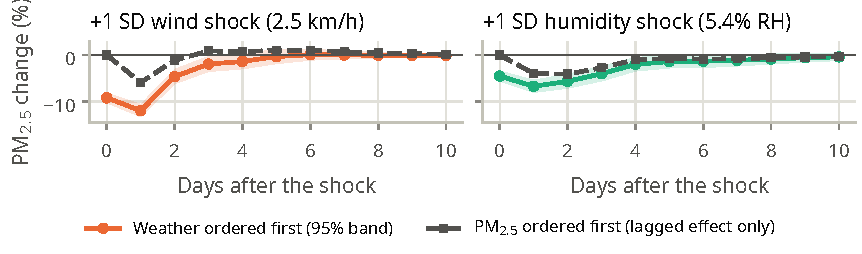
\includegraphics[width=\linewidth]{fig/irf_range.pdf}\\[3pt]
  \begin{defbox}{Impulse response.}
    The model's predicted path of \pmtwo{} after a one-SD shock. \textbf{Ordering:} weather first lets a shock move \pmtwo{} on the same day; \pmtwo{} first allows lagged effects only. We show both.
  \end{defbox}
  \begin{takeaway}
    A one-SD wind shock cuts \pmtwo{} by \irfWindA--\irfWindB\% the next day, humidity by \irfRhA--\irfRhB\%; both fade within about a week.
    Weekly: \emph{last} week's weather adds nothing to predict this week's \pmtwo{} ($p=\lagWindP$ wind, \lagRhP\ humidity).
  \end{takeaway}
\end{frame}

% ───────────────────────── 13. What we established ─────────────────────────
\begin{frame}{What We Have Established So Far}
  \begin{itemize}\setlength\itemsep{6pt}
    \item \textbf{Seasonality:} a strong yearly cycle ($F_S=\Fs$; winter \ratioWM$\times$ the monsoon), so the forecasting model must be seasonal ($s=52$ weeks).
    \item \textbf{Transformation:} the log stabilises the variance (monthly spread \sdRatioRaw$\times\to$\sdRatioLog$\times$, skewness \skewRaw\ $\to$ \skewLog); log \pmtwo{} is stationary on the training years, so $d=0$.
    \item \textbf{Causality:} wind and humidity \textbf{Granger-cause} \pmtwo{} (robust to lag choice, differencing, robust errors and a rain control); the reverse is absent for humidity and weak for wind.
    \item \textbf{Size and timing:} a one-SD shock lowers \pmtwo{} by \irfWindA--\irfWindB\% (wind) and \irfRhA--\irfRhB\% (humidity) the next day, fading within about a week.
    \item \textbf{Horizon:} last week's weather adds nothing for predicting this week's \pmtwo{} ($p\approx0.5$), so weather is a short-memory driver and the 12-month model should not rely on it.
  \end{itemize}
  \vspace{4pt}
  \begin{takeaway}
    Answer to Q1: \textbf{yes}, weather (wind, humidity) drives \pmtwo{} over the following days, which is the evidence that justifies testing weather inputs in the forecasting models next.
  \end{takeaway}
\end{frame}

% ───────────────────────── 14. Limits and next phase ─────────────────────────
\begin{frame}{Limits and Next Phase}
  \begin{columns}[T,onlytextwidth]
    \column{0.485\linewidth}
    \begin{card}[title={Limits to keep in mind}]{porange}\small
      \begin{itemize}\setlength\itemsep{3pt}
        \item Granger = predictive causality; mixing height, stubble burning and fireworks are not measured.
        \item Weather's share of 14-day forecast error depends on the VAR ordering: \fevdA--\fevdB\%.
        \item One city; data end in mid-2020.
      \end{itemize}
    \end{card}
    \column{0.485\linewidth}
    \begin{card}[title={Next phase (Q2: forecasting)}]{pblue}\small
      \begin{itemize}\setlength\itemsep{3pt}
        \item SARIMA(X): order search by AIC/BIC, residual checks (Ljung-Box, ARCH).
        \item Baselines: seasonal naive, climatology, Linear Regression, LSTM; compare test MAE on 2019.
        \item Final 12-month forecast with 95\% intervals and a monthly AQI advisory table; 2020 lockdown as a case study.
      \end{itemize}
    \end{card}
  \end{columns}
  \vspace{8pt}
  \centering
  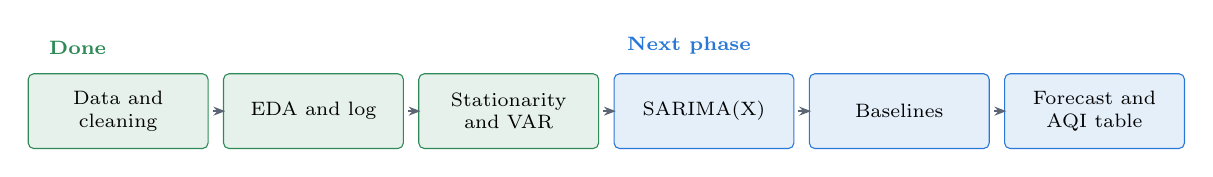
\begin{tikzpicture}[font=\scriptsize,x=1cm,y=1cm]
    \foreach \x/\c/\t in {1.1/pgreen/Data and cleaning, 3.58/pgreen/EDA and log, 6.06/pgreen/Stationarity and VAR, 8.54/pblue/SARIMA(X), 11.02/pblue/Baselines, 13.5/pblue/Forecast and AQI table}
      {\node[draw=\c,fill=\c!12,rounded corners=2pt,minimum width=2.2cm,minimum height=0.95cm,align=center,text width=2.05cm] at (\x,0) {\t};}
    \foreach \a in {2.3,4.78,7.26,9.74,12.22} {\draw[-{Stealth[length=1.5mm]},line width=0.7pt,graytxt] (\a,0) -- ++(0.16,0);}
    \node[text=pgreen,anchor=south west] at (0.1,0.6) {\textbf{Done}};
    \node[text=pblue,anchor=south west] at (7.44,0.6) {\textbf{Next phase}};
  \end{tikzpicture}
\end{frame}

% ───────────────────────── Backup A: glossary ─────────────────────────
\appendix
\begin{frame}{Backup: Glossary of Terms}
  \footnotesize
  \begin{columns}[T,onlytextwidth]
    \column{0.485\linewidth}
    \textbf{PM$_{2.5}$}: particles under 2.5 $\mu$m, \ugm{}.\\[2pt]
    \textbf{AQI}: India's Air Quality Index, CPCB categories.\\[2pt]
    \textbf{Reanalysis (ERA5)}: observations blended into a weather model.\\[2pt]
    \textbf{STL, $F_S$}: trend/seasonal/residual split; seasonal strength.\\[2pt]
    \textbf{Log transform}: makes percentage swings equal; stabilises variance.\\[2pt]
    \textbf{Volatility}: how much values swing; \textbf{ARCH-LM} tests clustering of big swings; \textbf{Levene} tests equal spread.\\[2pt]
    \textbf{Stationary}: no drift in mean, spread or autocorrelation; \textbf{ADF/KPSS} test it.
    \column{0.485\linewidth}
    \textbf{VAR}: each variable predicted from past values of all variables.\\[2pt]
    \textbf{Granger causality}: past X improves the forecast of Y.\\[2pt]
    \textbf{HAC errors}: standard errors robust to autocorrelation and changing variance.\\[2pt]
    \textbf{Shock}: the unpredictable part of a variable today; \textbf{SD} = its typical size.\\[2pt]
    \textbf{Impulse response}: path of PM$_{2.5}$ after a shock; \textbf{FEVD}: share of forecast error due to each variable.\\[2pt]
    \textbf{SARIMA(X)} (next phase): seasonal ARIMA, optionally with external regressors such as weather.
  \end{columns}
\end{frame}

% ───────────────────────── Backup B: robustness ─────────────────────────
\begin{frame}{Backup: How Robust Is the Weather Result?}
  \centering\scriptsize\setlength{\tabcolsep}{4pt}
  \begin{tabular}{|l|l|r|r|}
\hline
\textbf{Direction} & \textbf{Model} & \textbf{Wald $\chi^2$} & \textbf{$p$ (HAC)} \\\hline
Wind $\to$ PM$_{2.5}$ & PM$_{2.5}$, wind, humidity & 96.3 & $6.0\times10^{-20}$ \\\hline
Humidity $\to$ PM$_{2.5}$ & PM$_{2.5}$, wind, humidity & 54.8 & $3.5\times10^{-11}$ \\\hline
Wind $\to$ PM$_{2.5}$ & + rain control & 93.2 & $2.8\times10^{-19}$ \\\hline
Humidity $\to$ PM$_{2.5}$ & + rain control & 40.7 & $3.0\times10^{-8}$ \\\hline
Rain $\to$ PM$_{2.5}$ & + rain control & 1.2 & 0.88 \\\hline
PM$_{2.5}$ $\to$ Wind & PM$_{2.5}$, wind, humidity & 7.9 & 0.096 \\\hline
PM$_{2.5}$ $\to$ Humidity & PM$_{2.5}$, wind, humidity & 3.1 & 0.55 \\\hline
\end{tabular}
\par\vspace{2pt}
  \begin{tabular}{|l|c|c|c|c|}
\hline
\textbf{Shock} & \textbf{Day 1: W-first} & \textbf{Day 1: P-first} & \textbf{14-day share: W-first} & \textbf{14-day share: P-first} \\\hline
+1 SD wind shock & -12\% & -6\% & 20\% & 3\% \\\hline
+1 SD humidity shock & -7\% & -4\% & 10\% & 3\% \\\hline
\end{tabular}
\par
  {\tiny W-first = weather ordered first; P-first = PM$_{2.5}$ ordered first.}\par\vspace{1pt}
  \begin{takeaway}
    Robust (HAC) tests agree with the plain tests. The reverse direction (PM$_{2.5}$ $\to$ wind) is weakly significant at 1--2 lags only. The size of a shock's effect and weather's share of forecast error depend on the VAR ordering, so we report ranges, not single values.
  \end{takeaway}
\end{frame}

% ───────────────────────── Backup C: boxplot ─────────────────────────
\begin{frame}{Backup: PM$_{2.5}$ by Month}
  \centering
  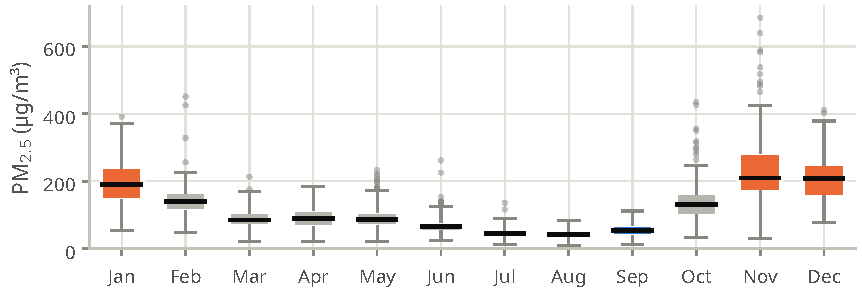
\includegraphics[width=\linewidth]{fig/seasonal_boxplot.pdf}\\[2pt]
  \begin{takeaway}
    Box = middle 50\% of days, line = median, dots = unusually high days. Orange: winter (Nov--Jan); blue: monsoon (Jul--Sep).
  \end{takeaway}
\end{frame}

\end{document}
